\section{IAFoosball}
IAFoosball is the name of the project and startup we developed in the previous semester. It is meant to make foosball more interactive, to show and share statistics, and make it more sociable by using new technologies. The planned services include global and private rankings, table finder, friends, automatic tournaments and more. Because it is part of an university project, we used the latest and greatest technology. The front end is written in Flutter and pReact, the back end is separated in containerized microservices written in Go and all communication is done through gRPC, which uses protobuffs and HTTP/2. \Cref{fig:architectureOld} shows this architecture.

\begin{figure}[h!]
    \centering
    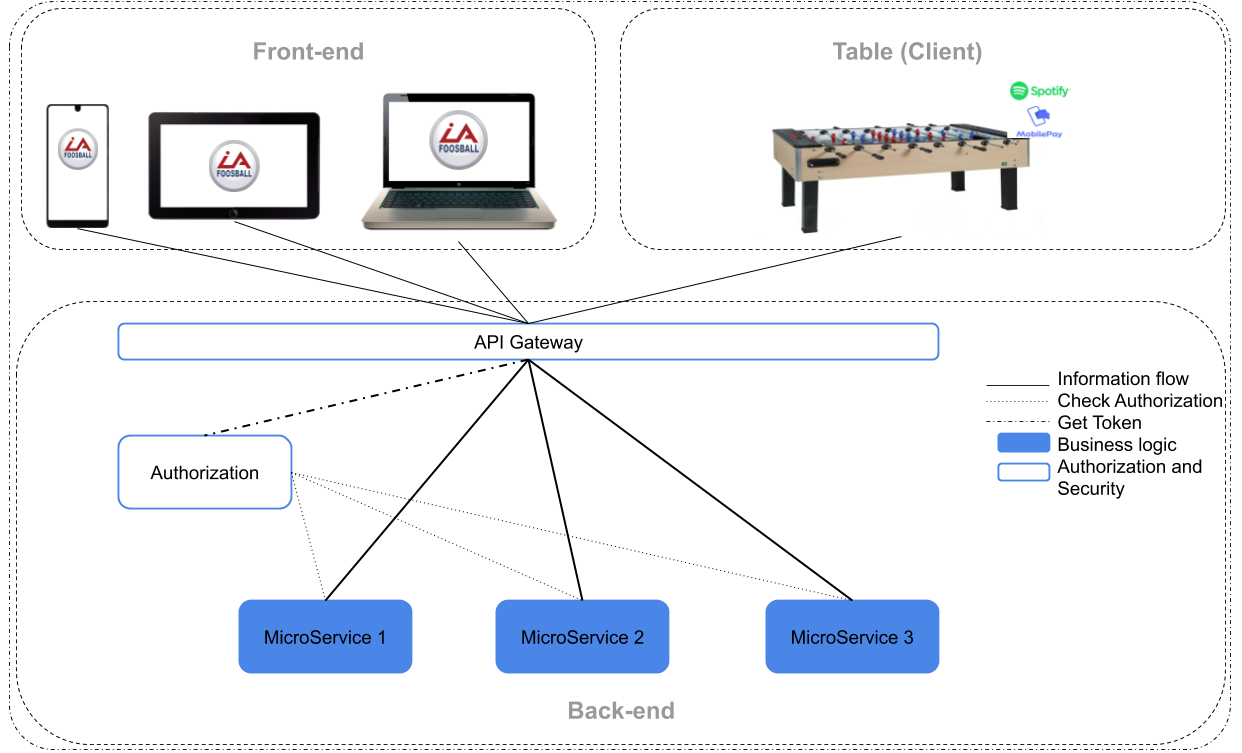
\includegraphics[scale=0.2]{figures/architecture-old.png}% picture filename
    \caption{The old IAFoosball architecture}\label{fig:architectureOld}
\end{figure}

The foosball table in \cref{fig:architectureOld} is the development version and has all features. It includes, speakers with Spotify integration, LED lights, automatic ball release and a tablet. However, the software and hardware power the table is not new  and not portable. To make IAFoosball more compelling for people and business which just want goal counting and possibly ball speed measurments, we wanted to cut down on features and instead concentrate on quality.\\


\subsection{Goal Design}
The goal design is the primary part of this report and in our opinion the most lacking part in the old setup. 
\Cref{fig:goalOld} shows the electronics of the old goal setup.

\begin{figure}[h!]
    \centering
    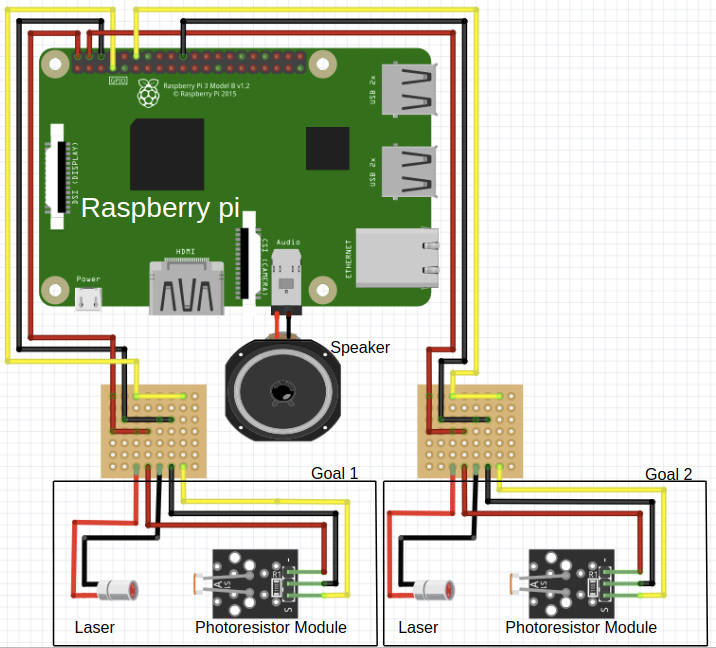
\includegraphics[scale=0.3]{figures/goal-old.png}
    \caption{The old IAFoosball goal}\label{fig:goalOld}
\end{figure}

The sensors were directly connected to raspberry pi and a simple javascript application registered the goals and send them to a remote server. This required a power outlet and a raspberry pi on each table. It also required cables from each goal to the raspberry pi. This approach did not scale well and in a multi-table setup also wasted money as each table needed its own raspberry pi. We re-thought the design, making it more varsatile, easier to integrate and manage and also cheaper for multiple tables.

\begin{figure}[h!]
    \centering
    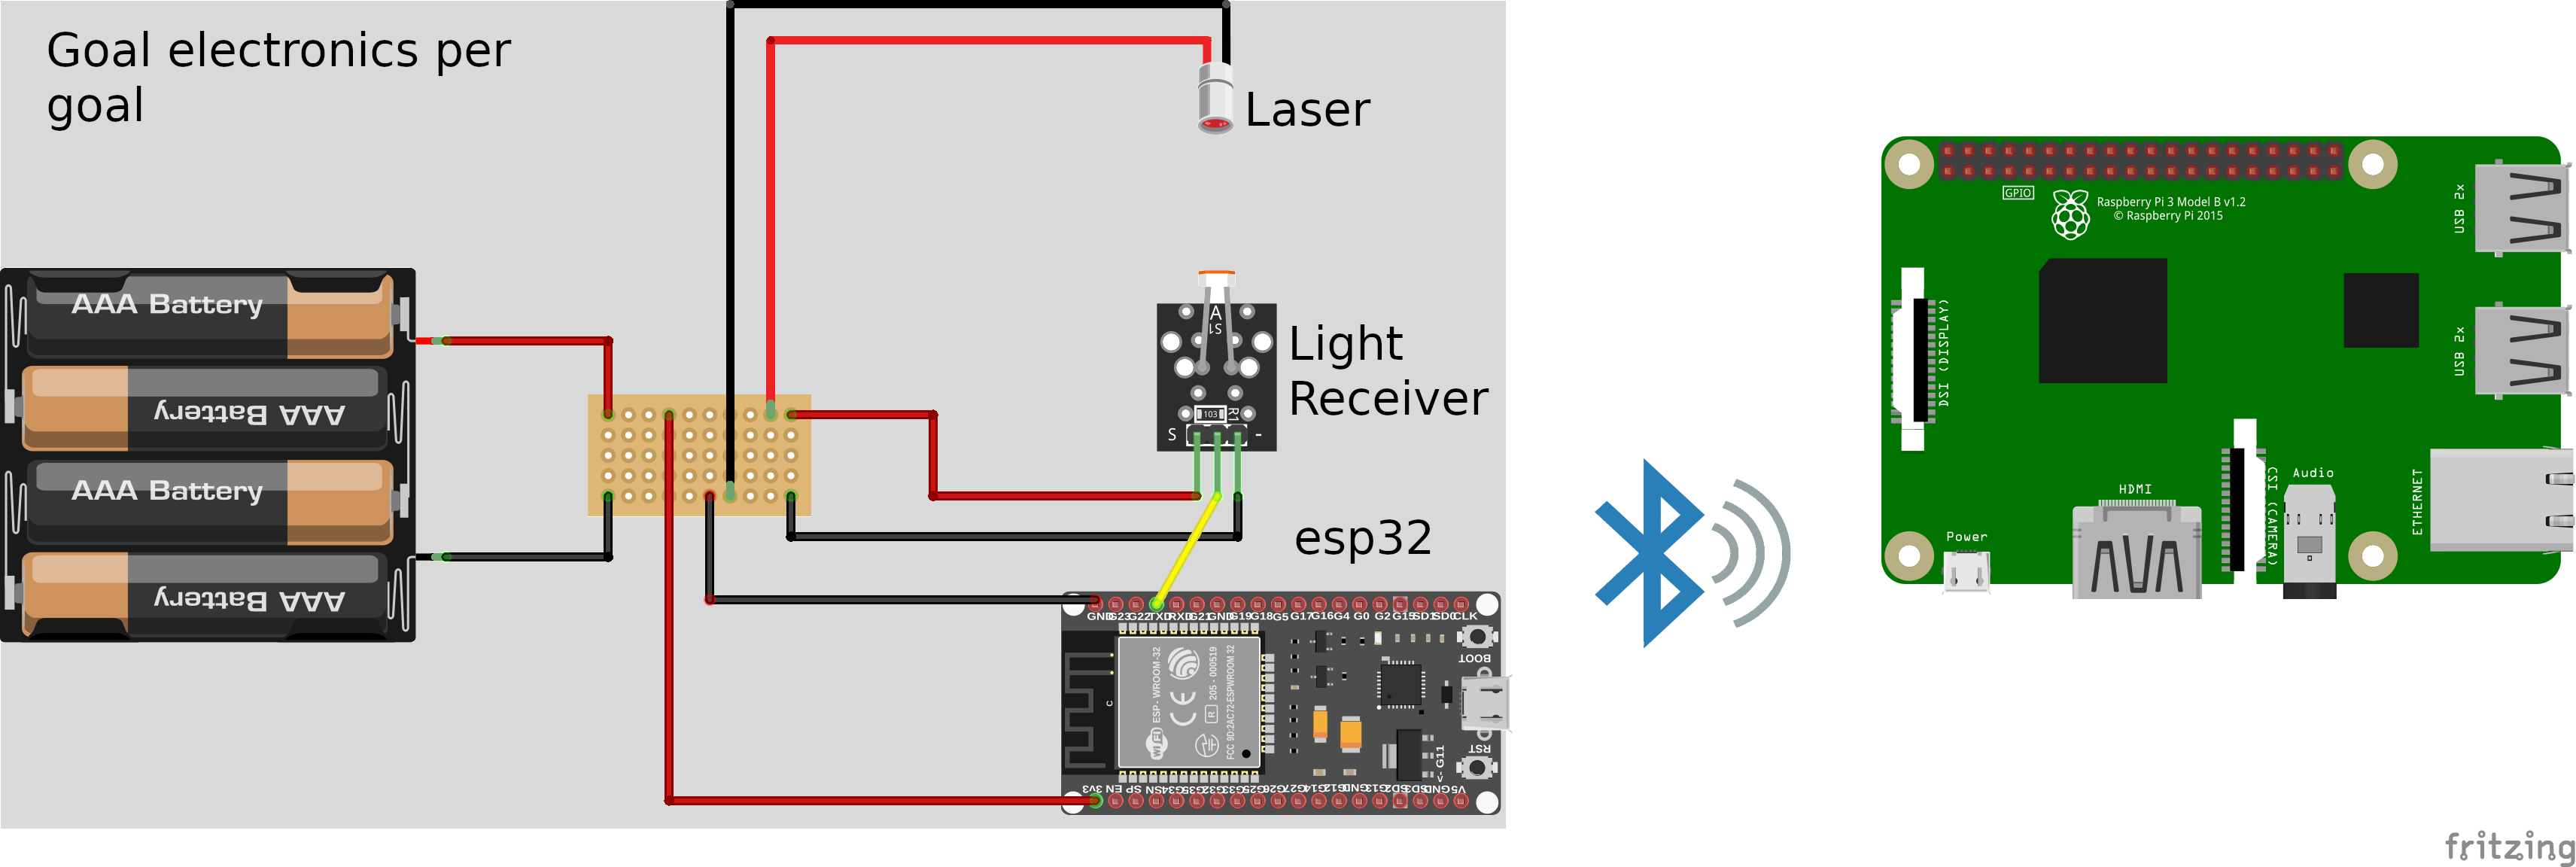
\includegraphics[scale=0.4]{figures/goal-new.png}% picture filename
    \caption{The new IAFoosball goal}\label{fig:goalNew}
\end{figure}

\Cref{fig:goalNew} shows this new setup. Marked in grey are the components used for each goal, a battery (we use a lithium-ion battery), one laser, one light sensor and one esp32. To measure goal speed we would need to have to lasers and two sensors. The esp32 is the component doing the computation and sending data to a raspberry pi via bluetooth low energy (BLE). It is powered by a battery pack and only active when the need arises.\\

